%\title{Using the forest package to create trees in LaTeX}
% From http://tex.stackexchange.com/a/108728/23931 
\documentclass[12pt,preview,border=0]{standalone}
\usepackage[paperheight=8cm,paperwidth=6cm]{geometry}
\usepackage{graphicx}
% \usepackage{forest}
\usepackage{amsmath}
% \usepackage{txfonts}  %pretty math font
\usepackage{kmath,kerkis}
\usepackage{tikz}
\usetikzlibrary{arrows,automata,positioning}

% fontspec requires xelatex/lualatex
% \usepackage{fontspec}
% \setmainfont[Scale=1,Ligatures={Common}]{Adobe Caslon Pro}
% \setromanfont[Scale=1,Ligatures={Common}]{Adobe Caslon Pro}

%%%%%% XeLaTeX Math Font Setup #%%%%%%%%%%%%%%
% \usepackage{bm}
% \usepackage{mathspec}
% \usepackage{xltxtra}  % also loads fontspec
% \usepackage{xunicode}
% \usepackage{fontspec}
% \defaultfontfeatures{Mapping=tex-text}
% \setmainfont[Scale=1,Ligatures={Common}]{Adobe Caslon Pro}
% \setromanfont[Scale=1,Ligatures={Common}]{Adobe Caslon Pro}
% \setmathrm[Scale=1]{Adobe Caslon Pro}
% \setmathfont(Digits,Latin)[Numbers={Lining,Proportional}]{Adobe Caslon Pro}
%%%%%%%%%%%%%%%%%%%%%%%%%%%%%%%%%%%%%%%%%%%%%%


%%%%%%%%%%%%%%%%%%%%%%%%%%%%%
% \usepackage{fontspec,mathfont}
% \setmainfont{Adobe Caslon Pro}
% % \setmathfont{Adobe Caslon Pro}
% \mathfont{Cambria Math}
%%%%%%%%%%%%%%%%%%%%%%%%%%%%%
\usetikzlibrary{backgrounds}

\begin{document} 
\begin{center}
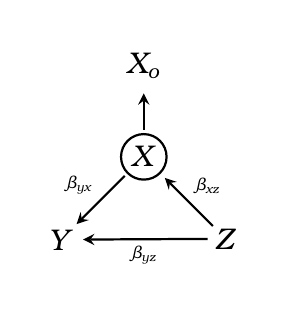
\begin{tikzpicture}[
	> = stealth, % arrow head style
	shorten > = 1pt, % don't touch arrow head to node
	auto,
	node distance = 2cm, % distance between nodes
	thick, % line style
	U/.style={circle, draw=black, inner sep=1.8pt, outer sep=1.5pt, minimum size=3mm, font=\large},  %draw=black, fill=white
	O/.style={circle, inner sep=1.4pt, outer sep=-.75pt, minimum size=3mm, font=\large},              %draw=white, fill=white
	background rectangle/.style={fill=white}, show background rectangle  % add backgroud
	]
	
	% Nodes and their relative positions
	% t = 0
    \node[U] (X) {$X$};	
    \node[O] (Xo) [above = .5 of X] {$X_{o}$};
    \node[O] (Z) [below right =.9 of X] {$Z$};
    \node[O] (Y) [below left = .9 of X] {$Y$};
       
	% Paths connecting nodes
    \path[->] (X) edge node[above left,scale=.7]{$~~\beta_{yx}$} (Y);
    \path[->] (X) edge (Xo);
    \path[->] (Z) edge node[above right,scale=.7]{$\beta_{xz}$} (X);
    \path[->] (Z) edge node[scale=.7]{$\beta_{yz}$} (Y);
\end{tikzpicture}

\end{center}

\end{document}
